\documentclass[tikz,border=2pt]{standalone}
\renewcommand{\familydefault}{\sfdefault}
\usetikzlibrary{arrows.meta,calc,positioning}
\tikzset{every picture/.style={line width=1pt, >=Stealth},
         hl/.style={fill=black, fill opacity=0.12, text opacity=1}}
\begin{document}
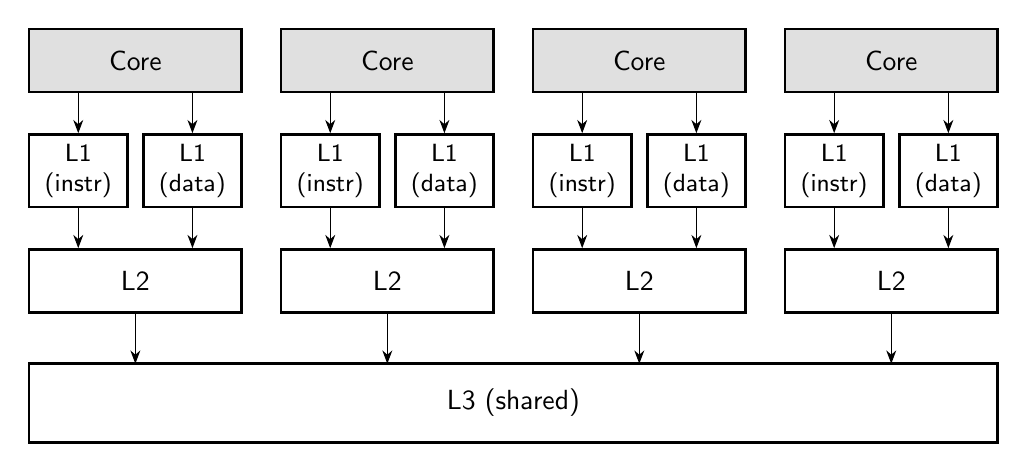
\begin{tikzpicture}[box/.style={draw, align=center, minimum height=0.8cm}, l1/.style={box, minimum width=1.25cm, font=\small}]
  % Each core has private L1 caches (split into instructions and data) and an L2; all cores share the L3.
  \foreach \c in {0, ..., 3} {
    \begin{scope}[xshift=3.2cm*\c]
      \node[box, hl, minimum width=2.7cm] (core\c) at (0, 0) {Core};
      \node[l1] (i\c) at (-0.725, -1.4) {L1 \\ (instr)};
      \node[l1] (d\c) at (0.725, -1.4) {L1 \\ (data)};
      \node[box, minimum width=2.7cm] (l2\c) at (0, -2.8) {L2};
      \draw[->, thin] (core\c.south -| i\c) -- (i\c);
      \draw[->, thin] (core\c.south -| d\c) -- (d\c);
      \draw[->, thin] (i\c) -- (l2\c.north -| i\c);
      \draw[->, thin] (d\c) -- (l2\c.north -| d\c);
      \draw[->, thin] (l2\c) -- (0, -3.85);
    \end{scope}
  }
  \node[box, minimum width=12.3cm, minimum height=1cm] at (4.8, -4.35) {L3 (shared)};
\end{tikzpicture}
\end{document}
